\documentclass[11pt,a4paper,twoside,openright]{report}

\usepackage[top=25mm,bottom=25mm,right=25mm,left=30mm,head=12.5mm,foot=12.5mm]{geometry}
\let\openright=\cleardoublepage

\usepackage[a-2u]{pdfx}

\usepackage[
   backend=biber
%  ,style=iso-authoryear
  ,style=alphabetic
  ,citestyle=numeric
  ,sortlocale=cs_CZ
  ,bibencoding=UTF8
  %,block=ragged
]{biblatex}
\addbibresource{references.bib}

%% Přepneme na českou sazbu, fonty Latin Modern a kódování češtiny
\usepackage[czech]{babel}
\usepackage{lmodern}
\usepackage[T1]{fontenc}
\usepackage{textcomp}
\usepackage[utf8]{inputenc}

% Set fonts
\RequirePackage[osf]{mathpazo} % Palatino with oldstyle figures
\newcommand\liningnums[1]{\fontfamily{ppl}\selectfont#1}
\RequirePackage{eulervm}
\RequirePackage[scaled=.8819]{sourcecodepro} % Source Code Pro typeface for monospace

%%% Další užitečné balíčky (jsou součástí běžných distribucí LaTeXu)
\usepackage{amsmath}        % rozšíření pro sazbu matematiky
\usepackage{amsfonts}       % matematické fonty
\usepackage{amsthm}         % sazba vět, definic apod.
\usepackage{bm}             % tučné symboly (příkaz \bm)
\usepackage{graphicx}       % vkládání obrázků
\usepackage{fancyvrb}       % vylepšené prostředí pro strojové písmo
\usepackage{fancyhdr}       % prostředí pohodlnější nastavení hlavy a paty stránek
\usepackage{icomma}         % inteligetní čárka v matematickém módu
\usepackage{dcolumn}        % lepší zarovnání sloupců v tabulkách
\usepackage{booktabs}       % lepší vodorovné linky v tabulkách
\makeatletter
\@ifpackageloaded{xcolor}{
   \@ifpackagewith{xcolor}{usenames}{}{\PassOptionsToPackage{usenames}{xcolor}}
  }{\usepackage[usenames]{xcolor}} % barevná sazba
\makeatother
\usepackage{multicol}       % práce s více sloupci na stránce
\usepackage{caption}
\usepackage{enumitem}
\usepackage{lipsum}
\setlist[itemize]{noitemsep, topsep=0pt, partopsep=0pt}
\setlist[enumerate]{noitemsep, topsep=0pt, partopsep=0pt}
\setlist[description]{noitemsep, topsep=0pt, partopsep=0pt}
\usepackage{pdfpages}

\usepackage{tocloft}
\setlength\cftparskip{0pt}
\setlength\cftbeforechapskip{1.5ex}
\setlength\cftfigindent{0pt}
\setlength\cfttabindent{0pt}
\setlength\cftbeforeloftitleskip{0pt}
\setlength\cftbeforelottitleskip{0pt}
\setlength\cftbeforetoctitleskip{0pt}
\renewcommand{\cftlottitlefont}{\Huge\bfseries}
\renewcommand{\cftloftitlefont}{\Huge\bfseries}
\renewcommand{\cfttoctitlefont}{\Huge\bfseries}

% vyznaceni odstavcu
\parindent=0pt
\parskip=11pt

% zakaz vdov a sirotku - jednoradkovych pocatku ci koncu odstavcu na prechodu mezi strankami
\clubpenalty=1000
\widowpenalty=1000
\displaywidowpenalty=1000

% nastaveni radkovani
\renewcommand{\baselinestretch}{1.20}

% nastavení hlavy a paty stránek
\fancyhf{}
\renewcommand{\chaptermark}[1]{\markboth{#1}{}}
\fancyhead[RO,LE]{\leftmark}
\fancyfoot[RO,LE]{\thepage}
%\renewcommand{\footrulewidth}{0pt}
\fancypagestyle{plain}{%
\fancyhf{} % clear all header and footer fields
\fancyfoot[RO,LE]{\thepage}
\renewcommand{\headrulewidth}{0pt}
%\renewcommand{\footrulewidth}{0.5pt}
}

% Tato makra přesvědčují mírně ošklivým trikem LaTeX, aby hlavičky kapitol
% sázel příčetněji a nevynechával nad nimi spoustu místa. Směle ignorujte.
\makeatletter
\def\@makechapterhead#1{
  {\parindent \z@ \raggedright 
   \Huge\bfseries \thechapter. #1
   \par\nobreak
   \vskip 20\p@
}}
\def\@makeschapterhead#1{
  {\parindent \z@ \raggedright 
   \Huge\bfseries #1
   \par\nobreak
   \vskip 20\p@
}}
\makeatother

% Trochu volnější nastavení dělení slov, než je default.
\lefthyphenmin=2
\righthyphenmin=2

% Zapne černé "slimáky" na koncích řádků, které přetekly, abychom si
% jich lépe všimli.
\overfullrule=1mm

%% Balíček hyperref, kterým jdou vyrábět klikací odkazy v PDF,
%% ale hlavně ho používáme k uložení metadat do PDF (včetně obsahu).
%% Většinu nastavítek přednastaví balíček pdfx.
\hypersetup{unicode}
\hypersetup{breaklinks=true}
\hypersetup{hidelinks}

%%% Prostředí pro sazbu kódu, případně vstupu/výstupu počítačových
%%% programů. (Vyžaduje balíček fancyvrb -- fancy verbatim.)

\DefineVerbatimEnvironment{code}{Verbatim}{fontsize=\small, frame=single}



\def\NazevPrace{Webová kalkulačka podílu jednotlivce na státním rozpočtu ČR}
\def\Trida{R8.A}
\def\AutorPrace{Tomáš Hozda}
\def\DatumOdevzdani{2023}

% Vedoucí práce: Jméno a příjmení s~tituly
\def\Vedouci{Bc. Emil Miler}

% Studijní program a obor
\def\StudijniProgram{studijní program}
\def\StudijniObor{studijní obor}

% Text čestného prohlášení
\def\Prohlaseni{Prohlašuji, že jsem svou práci vypracoval samostatně a použil jsem pouze prameny a literaturu
uvedené v~seznamu bibliografických záznamů. Nemám žádné námitky proti zpřístupňování této práce v~souladu se
zákonem č. 121/2000 Sb. o~právu autorském, o~právech souvisejících s~právem autorským a
o~změně některých zákonů (autorský zákon) ve znění pozdějších předpisů.}

% Text poděkování
\def\Podekovani{%
Rád bych poděkoval rodině, přátelům, vedoucímu práce
a bratrovi za konzultaci práce.
}

% Abstrakt česky
\def\Abstrakt{%
Cílem práce je vytvořit webovou aplikaci, která funguje jako kalkulačka podílu jednotlivce na státním rozpočtu ČR. Uživatel zadá své příjmy a výdaje (různé kategorie podle zdanění) a kalkulačka vypočítá, kolik peněz za daný rok odvedl do státní rozpočtu a jak s nimi stát naložil (za co je utratil). Aplikace spravuje databázi vybraných státních výdajů a zobrazí v přepočtu, jak se uživatel na nich podílel. Databázi výdajů stejně jako státní rozpočty a průměrné hodnoty pro dané roky je možné upravovat a přidávat skrze aplikaci. Aplikace se dokáže vypořádat i s faktem, když stát utratí více, než jsou jeho příjmy. Výsledkem tak je, že uživatel z vypočítané statistiky získá obrázek o tom, jaké množství peněz odvede státu, kolik je z nich reálného užitku a k jakému účelu.
}

% Abstrakt anglicky
\def\AbstraktEN{%
The goal of the project is to create a web application, that will serve as a calculator of an individual's participation in the state budget of Czech Republic. The user will
enter their income and expenses (different categories based on taxation), and the calculator will compute, how much of his money went into the state budget, and how the state used them (that is, what it spent the money on). The application manages a database of selected state investments, and displays, how the user participated on them. The database of expenses, just like budgets and average state levies is possible to modify, add, and delete through the web interface. The app has no issue with the possibility, that the state may spent more money, than is its income. The result is that the user gets a picture, of how much money is levied from them into the state budget, and how much of it has an actual use (and which uses those are).
}

% 3 až 5 klíčových slov
\def\KlicovaSlova{daně, web, aplikace, kalkulačka, Flask, AlpineJS, PicoCSS, Nix}
% 3 až 5 klíčových slov anglicky
\def\KlicovaSlovaEN{taxes, web, application, calculator, Flask, AlpineJS, PicoCSS, Nix}


\begin{document}

%%% Titulní strana práce a další povinné informační strany

%%% Titulní strana práce

\pagestyle{empty}
\pagenumbering{gobble}
\hypersetup{pageanchor=false}

\begin{center}
\LARGE
\textbf{GYMNASIUM JANA KEPLERA}\\
{\large Parléřova 2/118, 169 00 Praha 6}

\vspace{\stretch{3}}


\includegraphics[width=.3\textwidth]{img/logo}

\vspace{\stretch{3}}

{\Huge\bfseries\NazevPrace}

\vspace{8mm}
\mdseries{Maturitní práce}

\vspace{\stretch{8}}
\large
\begin{tabular}{rl}
Autor: & \AutorPrace \\
\noalign{\vspace{2mm}}
Třída: & \Trida\\
\noalign{\vspace{2mm}}
Školní rok: & 2020/2021\\
\noalign{\vspace{2mm}}
Předmět: & Informatika \\
\noalign{\vspace{2mm}}
Vedoucí práce: & \Vedouci \\
\end{tabular}

\vspace{20mm}
Praha, \DatumOdevzdani
\end{center}


\openright

%%% 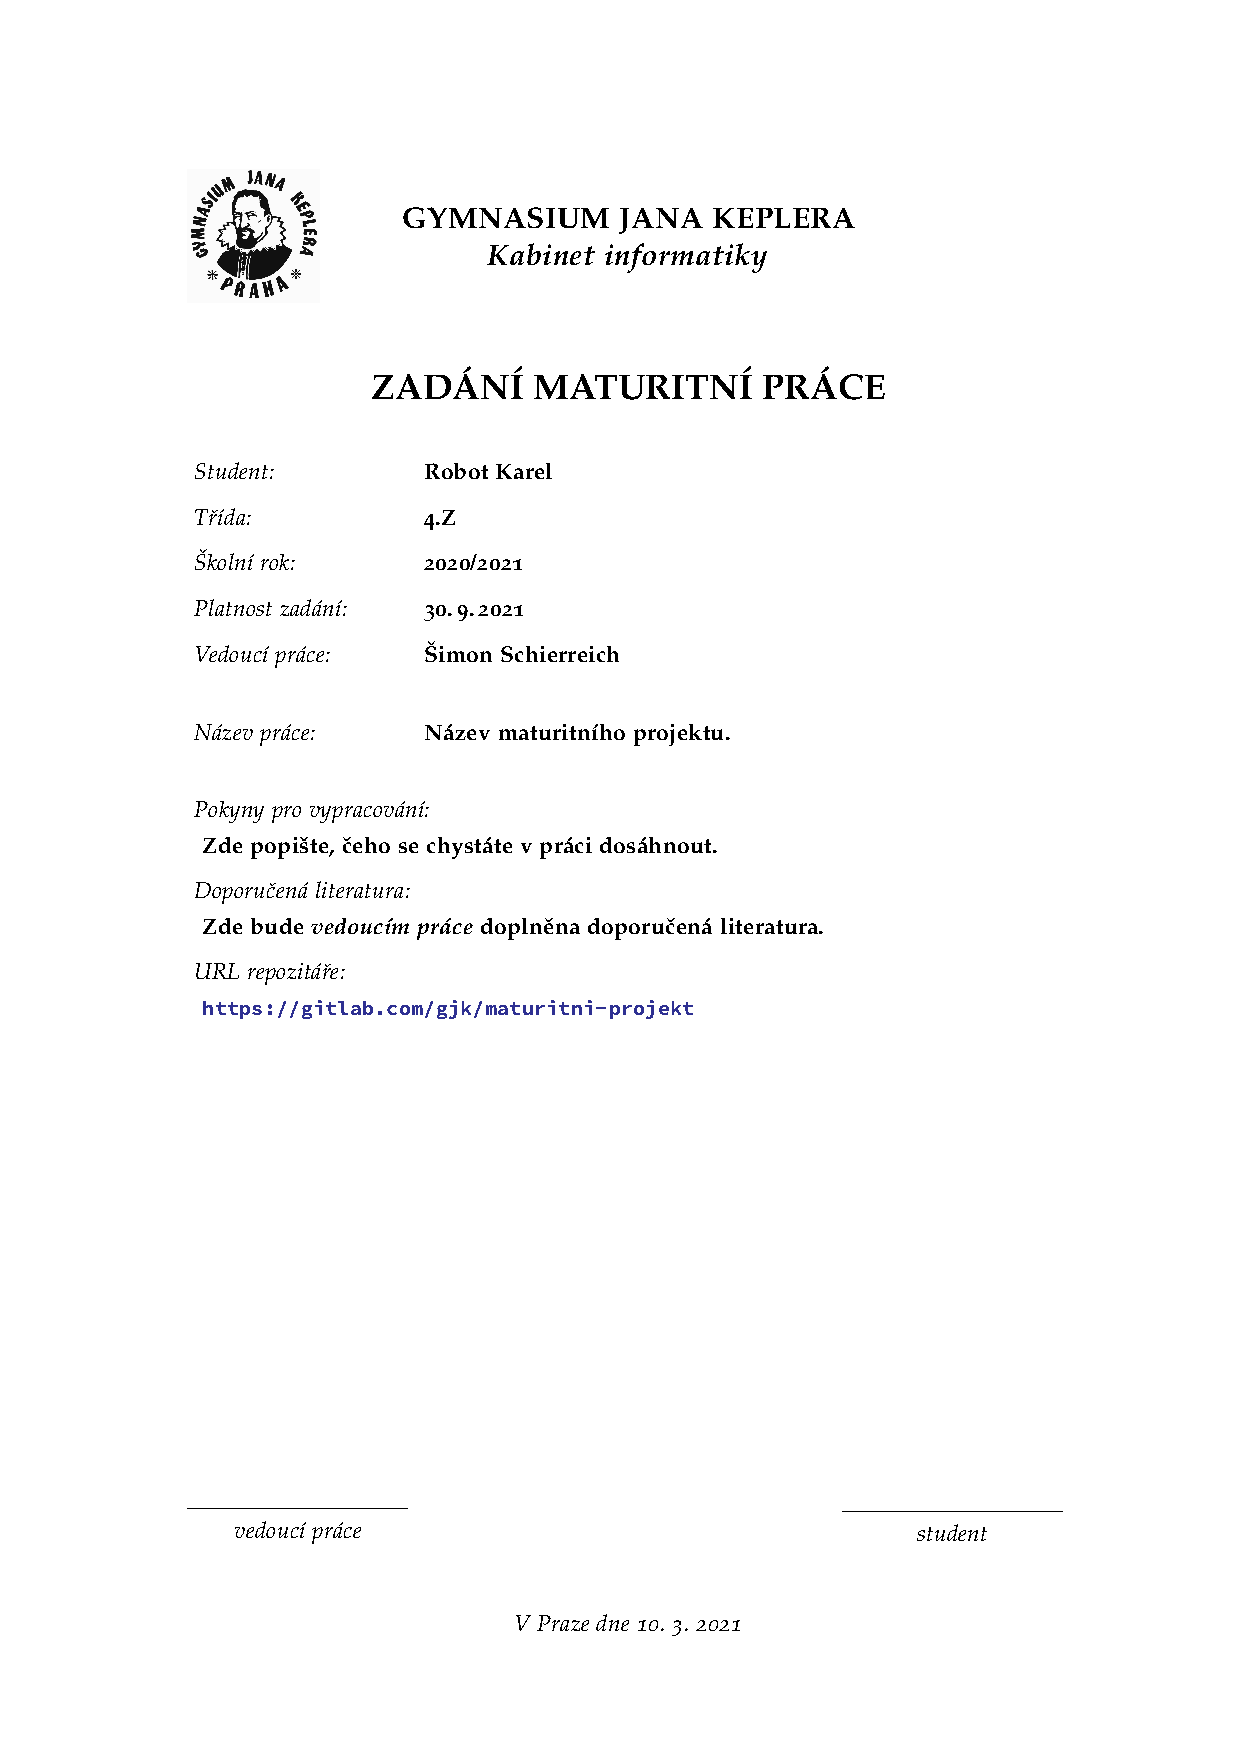
\includepdf[]{zadani.pdf}


%%% Strana s čestným prohlášením k bakalářské práci

\hypersetup{pageanchor=true}
\cleardoublepage
\vspace*{\fill}
\section*{Prohlášení}
\noindent
\Prohlaseni

\vspace{2cm}
\noindent
V Praze dne \today
\hspace*{\fill}\small{\AutorPrace}
\vspace{1cm}

%%% Poděkování
\openright
\vspace*{\fill}
\section*{Poděkování}
\noindent
\Podekovani
\vspace{1cm}


%%% Povinná informační strana bakalářské práce
\openright
\section*{Abstrakt}
\noindent
\Abstrakt
\subsection*{Klíčová slova}
\noindent
\KlicovaSlova

\vfill

\section*{Abstract}
\noindent
\AbstraktEN
\subsection*{Keywords}
\noindent
\KlicovaSlovaEN

\openright
\pagenumbering{arabic}

% Obsah
\setcounter{tocdepth}{2}
\tableofcontents

\chapter{Teoretická část}
\pagestyle{fancy}

V době, kdy jsem vymýšlel, co bych mohl vytvořit jako svůj maturitní projekt, se v médiích probírala možnost nákupu nových stíhacích letounů pro českou armádu. Odhadem se uváděla celková částka 48 miliard Kč. Slyšel jsem mnoho názorů o tom, jak moc peněz to je a že by bylo lepší peníze investovat jinam. Zamyslel jsem se tedy nad tím, kde stát peníze získává a za co je pak utrácí. V souvislosti s tím mě napadlo, kolik vlastně člověk sám odvede na daních do státního rozpočtu a jak by se tedy podílel na investicích a výdajích. 

Rozhodl jsem se tedy, že jako svůj maturitní projekt vytvořím webovou kalkulačku, která by se zabývala problematikou státního rozpočtu. Vytvořil jsem si představu, že uživatel do kolonek formuláře na webu zadá své příjmy a výdaje, kalkulačka údaje zpracuje a vypočítá z nich, kolik uživatel odvedl celkově za rok, který si vybere v nabídce, korun do státního rozpočtu. Uživatel by na stránce měl mít možnost prohlížet si údaje o státním rozpočtu z nabídky zpracovaných let. Dále jsem chtěl, aby kalkulčka zobrazila, prostřednitcvím jakých daní uživatel peníze státu odvedl. Tyto údaje by měly být společně v tabulce s celkovými státními příjmy. Vedle zobrazení státních výdajů jsem chtěl pak zobrazit údaje o tom, jak se uživatelem odvedená částka rozpočítala na výdaje. Dále jsem na webu chtěl uvést některé konkrétní investice státu, kolik za ně stát utratil a jak se na nich podílel uživatel. Pro lepší celkovou funkcionalitu kalkulačky jsem se rozhodl, že kalkulačka musí mít i správu databáze údajů, které zobrazuje.

Z teoretické části jsem se tedy musel zaměřit především na daňový systém a údaje o státním rozpočtu. K tomu jsem také musel dohledat konktrétní investice státu a všechny tyto části spojit funkčně do sebe. Pro vytvoření funkční kalkulačky jsem tedy potřeboval získat údaje o státním rozpočtu za vybrané roky, údaje o konkrétních investicích, od uživatele přijmout údaje o jeho příjmech a výdajích a podle pravidel daňového systému vypočítat jeho podíl, který by pak kalkulačka rozložila mezi jednotlivé výdaje a investice.

\section{Státní rozpočet}

Svojí teoretickou analýzu jsem začal hledáním údajů o státním rozpočtu. Stát musí být v těchto záležitostech transparentní, a tak na webu ministerstva financí jsou k dispozici tabulky plnění státního rozpočtu, které uvádí jenotlivé důležité položky příjmů a výdajů státního rozpočtu. U každé položky je uvedeno, jaká hodnota se pro daný rok očekávala a jaká finálně hodnota skutečně byla. Já jsem samozřejmě pracoval se skutečnými hodnotami, aby kalkulačka byla přesnější. Rozhodl jsem se pro práci s údaji z let 2020, 2021 a 2022, protože v době dokončení projektu mají již vyplněné skutečné údaje. Počítal jsem s tím, že v rámci správy databáze bude pak možné přidat údaje i pro jiné roky.

Tyto údaje jsem si potřeboval pouze přepsat do databáze. Z počátku jsem byl sice zmatený tím, že v souboru s údaji bylo více tabulek a uváděly různé příjmy. Na internetu jsem však poté dohledal, že existuje rozpočtové určení daní. Částka, kterou daňový poplatník odvede na daních, nemíří pouze do státního rozpočtu, ale dělí se. Část putuje do rozpočtu obcí, část do krajských rozpočtů a teprve zbytek skončí ve státním rozpočtu. Některé daně se dokonce odvádí pouze do obecních a krajských rozpočtů. Veřejné zdravotní pojištění se také nepočítá do příjmů státního rozpočtu. Pochopil jsem tedy, že do databáze si potřebuji vypsat údaje z tabulky, která zohledňuje opravdu pouze příjmy státního rozpočtu a ne celkové daňové příjmy.

\section{Konkrétní státní investice}

Vedle údajů o státním rozpočtu jsem také potřeboval získat příklady konkrétních investic a jejich náklady. Myslím si, že pro uživatele jsou snadno představitelnější a pochopitelnější konkrétní invesitce (např. nákup stíhacích letounů nebo dostavba Pražského okruhu) než obecné pojmy státních výdajů (např. neinvestiční transfery rozpočtům územní úrovně nebo ostatní běžné výdaje). Velmi dobře mi v tomto ohledu pomohl národní investiční plán na roky 2020 až 2050. Plán jsem projel a vybral jsem si z něj důležité a velké investice, které jsem zapsal do databáze. Samozřejmě je možné přidávat další investice z plánu skrze správu databáze aplikace.

Při vybíraní investic z plánu jsem si ale uvědomil problém složitosti výpočtu podílu jednotlivce na těchto investicích. Investice se většinou realizují mnoho let a není jasné, jakým přesným způsobem je stát financuje. Moje aplikace pracuje vždy s údaji za jeden rok a sice z celkových výdajů státního rozpočtu vím, kolik putovalo na investice, ale nevím kolik na jaké. Rozhodl jsem se tedy, že pro výpočet budu vycházet z předpokladu, že investice se celá realizovala a zaplatila pouze v roce, pro který si uživatel počítá své odvody a zobrazuje údaje o státním rozpočtu. U konkrétní investice by se tak zobrazil procentuální podíl na celkové částce, která za daný rok mířila na investice a podle toho částka, jakou by se uživatel podílel. Nejedná se tak o reálnou částku, ale i tak poskytuje představu o nákladnosti investice a velikosti podílu uživatele aplikace.

\section{Výpočet celkové odvedené částky na daních}

S již získanými obecnými informacemi o státních rozpočtech jsem se mohl zaměřit přímo na jednotlivce. Částku, kterou odvede do státního rozpočtu, musím určit z údajů, které mi poskytne. Potřeboval jsem si tedy rozmyslet, které údaje pro výpočet potřebuji od uživatele požadovat. Zaměřil jsem se tedy na státní příjmy a podíval se, které daně přinaší peníze do rozpočtu. Z těch jsem si vybral ty, na kterých se podílí jednotlivec sám - DPH, daň z příjmu fyzických osob, pojistné na sociální zabezpečení, daň z hazardu a spotřební daň z paliva, tabáku a alkoholu. Podle toho jsem si určil, jaké údaje od uživatele budu požadovat, abych konkrétní daň vypočítal.

\subsection{DPH}

DPH se dělí podle procentuálního odvodu do tří kategorií - základní sazba, první snížená sazba a druhá snížená sazba. V druhé snížené sazbě se odvádí daň ve výši 10\% a to především z vodného a stočného, nákupu knih, hudby, léků a z ubytovacích služeb. V první snížené sazbě to je 15\% a vyměřuje se pro potraviny a gastronomické služby, veřejnou dopravu a léčební pomůcky. Základní sazba je 21\% a vztahuje se na všechny ostatní nákupy a útraty. Od uživatele tedy potřebuji zjistit, kolik průměrné měsíčně utratí za dané kategorie.

\subsection{Daň z příjmu}

Daň z příjmu fyzických osob se dnes vypočítává z hrubého příjmu. Z hrubého příjmu tvoří 15\%. Výpočet probíhá tak, že si spočítáme 15\% z hrubého příjmu a odečteme od toho slevu na poplatníka - 2570 Kč měsíčně. Do roku 2020 se daň vypočítávala ze superhrubé mzdy - 15\% z 1.338násobku hrubé mzdy. Pokud si poplatník nárokuje slevu na dítě, odečte se i ta. Sleva na první dítě je 15204 Kč za rok, na druhé 22320 Kč za rok a na každé další 27840 Kč za rok. Dříve byl maximální součet omezen na 60300 Kč za rok, od roku 2022 sleva na děti nemá horní hranici. Ze slevy na děti je možné vyměřit daňový bonus. Tedy pokud sleva na děti převyšuje daň z příjmů, stát musí uhradit daňovému plátci rozdíl. V extrémních případech může stát díky slevě na děti zaplatit jednotlivici více, než by jinak jednotlivec celkově dovedl do státního rozpočtu. Na slevu má nárok pouze jeden z rodičů. K dani z příjmů patří ještě daň z kapitálových příjmů. To je také 15\%, ale vyměřuje se pouze, pokud za rok plátce zaznamená zisk z kapitálových příjmů vyšší než 100000 Kč. Pro výpočet musí uživatel zadat svůj hrubý příjem, počet dětí, pokud uplatňuje slevu na děti, a kapitálové příjmy.

\subsection{Sociální pojištění}

Při výpočtu odvodu na sociální pojištění záleží na tom, jestli je uživatel zaměstnanec nebo OSVČ. Výpočet se podle toho liší. V případě OSVČ jsem se rozhodl částku nepočítat, protože nevím, z jakého vyměřovacího základu si to uživatel počítá. Po uživateli, který je OSVČ, tedy požaduju, aby vyplnil kolonku s tím, kolik si na pojištění platí. Stejně tak požaduji, aby kolonku vyplnili ti, co pracují jako zaměstnanci, ale na zkrácený úvazek. Opět nevím, z čeho bych daň vypočítal. Pro klasické zaměstnance je to pak jednoduché. Zaměstnanec  na sociální pojištění sám odvádí 6,5\% ze své hrubé mzdy a k tomu za něj zaměstnavatel odvádí ještě 24,8\% z hrubé mzdy. Ve své aplikaci zohleňuji i peníze odvedené zaměstnavatelem, protože je také vnímám jako odměnu za práci zaměstnance.

\subsection{Spotřební daně a daň z hazardu}

Daň z hazardu je 23\%, spotřební daň z paliv je v průměru 11,5 Kč/l, spotřební daň z piva je 0,32 Kč/l, spotřební daň z lihovin je 322,5 Kč na litr ethanolu a spotřební daň za jednu cigaretu je 2,9 Kč. Uživatel tedy do kolonek zadá průměrnou částku, kterou prohraje na hazardu, kolik utratí za paliva, kolik vypije piva a lihovin a kolik vykouří cigaret za měsíc.

\subsection{Finální částka}

V instrukcích jsem upřesnil, že uživatelé mají do každé kolonky vyplnit průměrnou měsíční hodnotu údaje. Pomocí výše uvedených procentuálních sazeb kalkulačka spočítá kolik peněz uživatel odvedl na daních za vybrané položky a samozřejmě to vynásobí dvanácti, aby výsledkem byl údaj za celý rok. U vybraných daní také zohlední rozpočtové určení daní. Z prostředků odvedených prostřednictvím DPH a daně z příjmu fyzických osob míří do státního rozpočtu pouze 64,38\%. U daně z hazardu je to 70\%. Výsledkem výpočtů je celková částka, kterou uživatel za rok odvedl do státního rozpočtu.

\section{Rozbor uplatnění odvedené částky}

Pokud má aplikace údaje o státním rozpočtu, konktérních investicích a částku zaplacenou uživatelem nad daních, může začít zobrazovat informace o uplatnění odvedených peněz. V úvodu teoretické analýzy jsem uvedl, co by kalkulačka měla zobrazovat - kolik prostřednictvím jakých daní uživatel odvedl do rozpočtu, jak se peníze přerozdělily na výdaje a jak by se uživatel hypoteticky podílel na konkrétních investicích.

\subsection{Analýza kompozice odvedené částky}

Uživateli se vedle položek státních příjmů zobrazí, kolika korunami se na této položce podílel. Výpočet odpovídá postupům, které jsem uvedl u výpočtu celkové částky. Pouze zde aplikace zobrazuje částky odvedené na jednotlivých daní a nesčítá je.

\subsection{Analýza reálného uplatnění odvedené částky}

Uživateli se vedle položek státních výdajů zobrazí, kolika korunami se na této položce podílel. Výpočet je velmi jednoduchý. U každé položky aplikace vypočítá, jaký podíl položka tvoří z celkových výdajů. Toto procento aplikuje pak na částku odvedenou uživatelem na daních. Částka se tedy rozpočítá mezi jednotlivé položky ve stejném poměru, jako je to u celkových státních výdajů.

\subsection{Hypotetický podíl na konkrétních investicích}

Zde kalkulačka vezme celkové náklady konkrétní investice a spočítá, jaký procentuální podíl by náklady tvořily z peněz vyčleněných na investice za daný rok. Korunový podíl uživatele je výsledkem násobení vypočteného procenta a částky, kterou uživatel odvedl na daních a putovala na investice. V sekci 1.2 vysvětluji nepřesnosti tohoto výpočtu.

\chapter{Implementace}

Druhá kapitola obsahuje detailní informace o tom, jak probíhala implementace. Zde se objeví zdůvodnění výběru technologií, řešení problémů, na které jste narazili, informace o použitých knihovnách apod. Pochvalte se, nikdo to za Vás neudělá. Přiznejte chyby, není to ostuda.

\section{Ukázka sekce}

\lipsum

\chapter{Technická dokumentace}

\section{Požadavky}
Projekt je možné zprovoznit dvěma způsoby, za použití Nixu a bez něj. Postup s použitím Nixu je jednodušší a spolehlivější,
ale je použitelný pouze na Linuxových distribucích (a případně Macu), protože pro Windows nemá Nix podporu.

S Nixem jsou závislosti pro spuštění následující:

\begin{itemize}
\item Rozumná Linuxová distribuce (nebo MacOS)
\item \href{https://nixos.org/}{Nix}
\end{itemize}

V případě postupu bez Nixu je možné použít i Windows, ale je zapotřebí explicitně nainstalovat více závislostí:

\begin{itemize}
\item Python 3 (projekt byl vyvíjen s Pythonem 3.10.9, ale neměly by být problémy s kompatibilitou s novějšími verzemi)
\item PocketBase
\item \href{https://flask.palletsprojects.com/en/2.2.x/}{Flask}
\item \href{https://pypi.org/project/waitress/}{waitress} (na deployment)
\end{itemize}

Následující instrukce jsou pro Linuxové operační systémy, jakožto pro platformu, která se nejvíc hodí
na vývoj a provoz aplikací.

\subsection{Nix}
Nix je možné nainstalovat pomocí balíčkovače na vaší distribuci, například:

\begin{verbatim}
# debianovité
sudo apt-get install nix

# archovité
sudo pacman -S nix

# void linux
sudo xbps-install -Sy nix
\end{verbatim}

Doporučený je ale způsob z webové stránky Nixu\footnote{\url{https://nixos.org}}, který nainstaluje
Nix přes Nix:

\begin{verbatim}

\end{verbatim}

\subsection{Python}

\subsection{PocketBase}

\subsection{Flask}

\subsection{waitress}

\section{Instalace a spouštění}
\section{Uživatelská dokumentace}
Poslední kapitola obsahuje informace o tom, jak projekt, který v rámci maturitní práce vznikl, nainstalovat, spustit a používat.

\section{Ukázka sekce}


\subsection{A jedné podsekce}

\lipsum

\section{A další sekce}

\lipsum

\chapter*{Závěr}
\pagestyle{empty}
\addcontentsline{toc}{chapter}{Závěr}

Závěr obsahuje shrnutí práce a vyjadřuje se k míře splnění jejího zadání. Dále by se zde mělo objevit sebehodnocení studenta a informace o tom, co nového se naučil a jak vnímal svou práci na projektu.

%%% Seznam použité literatury
\nocite{einstein}\nocite{latexcompanion}\nocite{knuthwebsite}
\printbibliography[title={Seznam použité literatury},heading={bibintoc}]

%%% Seznam obrázků
\openright
\listoffigures
\addcontentsline{toc}{chapter}{Seznam obrázků}

%%% Seznam tabulek
\clearpage
\listoftables
\addcontentsline{toc}{chapter}{Seznam tabulek}

%%% Přílohy k práci, existují-li. Každá příloha musí být alespoň jednou
%%% odkazována z vlastního textu práce. Přílohy se číslují.

%\part*{Přílohy}
%\appendix

\end{document}
